% This document is licensed under:
% Creative Commons NonCommercial-Attribution-ShareAlike
% 2020
% Author: Spacial
% spacial_AT@gmail_DOT_com
\documentclass[a4paper,12pt]{article}
\usepackage[utf8]{inputenc}
\usepackage[T1]{fontenc}
\usepackage[brazil]{babel}
\usepackage{amsmath}
\usepackage{amsfonts}
\usepackage{amssymb}
\usepackage{graphicx}
\usepackage{hyperref}
\hypersetup{pdfstartview = {XYZ null null 1.00}}
\usepackage[hmargin=2cm,vmargin=3cm]{geometry}
\usepackage{wrapfig}
\usepackage{enumitem}
\usepackage{fancyhdr}
\usepackage{float}
\usepackage{eurosym}
\usepackage{abnt}
\pagestyle{fancy}
\usepackage[printwatermark]{xwatermark}
\usepackage{lastpage}
\usepackage{graphicx}
\usepackage[
type={CC},
modifier={by-nc-sa},
version={4.0},
]{doclicense}
\usepackage{fontawesome5}
\newcommand{\hsp}{\hspace{20pt}}
\newcommand{\HRule}{\rule{\linewidth}{0.5mm}}
\newwatermark[allpages,color=gray!5,angle=45,scale=3,xpos=0,ypos=0]{Regressão Não-Linear\\ \texttt{CC by-nc-sa 4.0}}
\usepackage{listings}

\lstset{language=Rlang,
basicstyle=\small\ttfamily,
stringstyle=\color{red},
otherkeywords={0,1,2,3,4,5,6,7,8,9},
morekeywords={abbreviate,abline,abs,acos,acosh,action,add1,add,%
aggregate,alias,Alias,alist,all,anova,any,aov,aperm,append,apply,%
approx,approxfun,apropos,Arg,args,array,arrows,as,asin,asinh,%
atan,atan2,atanh,attach,attr,attributes,autoload,autoloader,ave,%
axis,backsolve,barplot,basename,besselI,besselJ,besselK,besselY,%
beta,binomial,body,box,boxplot,break,browser,bug,builtins,bxp,by,%
c,C,call,Call,case,cat,category,cbind,ceiling,character,char,%
charmatch,check,chol,chol2inv,choose,chull,class,close,cm,codes,%
coef,coefficients,co,col,colnames,colors,colours,commandArgs,%
comment,complete,complex,conflicts,Conj,contents,contour,%
contrasts,contr,control,helmert,contrib,convolve,cooks,coords,%
distance,coplot,cor,cos,cosh,count,fields,cov,covratio,wt,CRAN,%
create,crossprod,cummax,cummin,cumprod,cumsum,curve,cut,cycle,D,%
data,dataentry,date,dbeta,dbinom,dcauchy,dchisq,de,debug,%
debugger,Defunct,default,delay,delete,deltat,demo,de,density,%
deparse,dependencies,Deprecated,deriv,description,detach,%
dev2bitmap,dev,cur,deviance,off,prev,,dexp,df,dfbetas,dffits,%
dgamma,dgeom,dget,dhyper,diag,diff,digamma,dim,dimnames,dir,%
dirname,dlnorm,dlogis,dnbinom,dnchisq,dnorm,do,dotplot,double,%
download,dpois,dput,drop,drop1,dsignrank,dt,dummy,dump,dunif,%
duplicated,dweibull,dwilcox,dyn,edit,eff,effects,eigen,else,%
emacs,end,environment,env,erase,eval,equal,evalq,example,exists,%
exit,exp,expand,expression,External,extract,extractAIC,factor,%
fail,family,fft,file,filled,find,fitted,fivenum,fix,floor,for,%
For,formals,format,formatC,formula,Fortran,forwardsolve,frame,%
frequency,ftable,ftable2table,function,gamma,Gamma,gammaCody,%
gaussian,gc,gcinfo,gctorture,get,getenv,geterrmessage,getOption,%
getwd,gl,glm,globalenv,gnome,GNOME,graphics,gray,grep,grey,grid,%
gsub,hasTsp,hat,heat,help,hist,home,hsv,httpclient,I,identify,if,%
ifelse,Im,image,\%in\%,index,influence,measures,inherits,install,%
installed,integer,interaction,interactive,Internal,intersect,%
inverse,invisible,IQR,is,jitter,kappa,kronecker,labels,lapply,%
layout,lbeta,lchoose,lcm,legend,length,levels,lgamma,library,%
licence,license,lines,list,lm,load,local,locator,log,log10,log1p,%
log2,logical,loglin,lower,lowess,ls,lsfit,lsf,ls,machine,Machine,%
mad,mahalanobis,make,link,margin,match,Math,matlines,mat,matplot,%
matpoints,matrix,max,mean,median,memory,menu,merge,methods,min,%
missing,Mod,mode,model,response,mosaicplot,mtext,mvfft,na,nan,%
names,omit,nargs,nchar,ncol,NCOL,new,next,NextMethod,nextn,%
nlevels,nlm,noquote,NotYetImplemented,NotYetUsed,nrow,NROW,null,%
numeric,\%o\%,objects,offset,old,on,Ops,optim,optimise,optimize,%
options,or,order,ordered,outer,package,packages,page,pairlist,%
pairs,palette,panel,par,parent,parse,paste,path,pbeta,pbinom,%
pcauchy,pchisq,pentagamma,persp,pexp,pf,pgamma,pgeom,phyper,pico,%
pictex,piechart,Platform,plnorm,plogis,plot,pmatch,pmax,pmin,%
pnbinom,pnchisq,pnorm,points,poisson,poly,polygon,polyroot,pos,%
postscript,power,ppoints,ppois,predict,preplot,pretty,Primitive,%
print,prmatrix,proc,prod,profile,proj,prompt,prop,provide,%
psignrank,ps,pt,ptukey,punif,pweibull,pwilcox,q,qbeta,qbinom,%
qcauchy,qchisq,qexp,qf,qgamma,qgeom,qhyper,qlnorm,qlogis,qnbinom,%
qnchisq,qnorm,qpois,qqline,qqnorm,qqplot,qr,Q,qty,qy,qsignrank,%
qt,qtukey,quantile,quasi,quit,qunif,quote,qweibull,qwilcox,%
rainbow,range,rank,rbeta,rbind,rbinom,rcauchy,rchisq,Re,read,csv,%
csv2,fwf,readline,socket,real,Recall,rect,reformulate,regexpr,%
relevel,remove,rep,repeat,replace,replications,report,require,%
resid,residuals,restart,return,rev,rexp,rf,rgamma,rgb,rgeom,R,%
rhyper,rle,rlnorm,rlogis,rm,rnbinom,RNGkind,rnorm,round,row,%
rownames,rowsum,rpois,rsignrank,rstandard,rstudent,rt,rug,runif,%
rweibull,rwilcox,sample,sapply,save,scale,scan,scan,screen,sd,se,%
search,searchpaths,segments,seq,sequence,setdiff,setequal,set,%
setwd,show,sign,signif,sin,single,sinh,sink,solve,sort,source,%
spline,splinefun,split,sqrt,stars,start,stat,stem,step,stop,%
storage,strstrheight,stripplot,strsplit,structure,strwidth,sub,%
subset,substitute,substr,substring,sum,summary,sunflowerplot,svd,%
sweep,switch,symbol,symbols,symnum,sys,status,system,t,table,%
tabulate,tan,tanh,tapply,tempfile,terms,terrain,tetragamma,text,%
time,title,topo,trace,traceback,transform,tri,trigamma,trunc,try,%
ts,tsp,typeof,unclass,undebug,undoc,union,unique,uniroot,unix,%
unlink,unlist,unname,untrace,update,upper,url,UseMethod,var,%
variable,vector,Version,vi,warning,warnings,weighted,weights,%
which,while,window,write,\%x\%,x11,X11,xedit,xemacs,xinch,xor,%
xpdrows,xy,xyinch,yinch,zapsmall,zip,TRUE,FALSE},%
otherkeywords={!,!=,~,\$,*,\&,\%/\%,\%*\%,\%\%,<-,<<-,_,/},%
deletekeywords={data,frame,length,as,character},
keywordstyle=\color{blue},
otherkeywordstyle=\color{red},
commentstyle=\color{gray},
}

\usepackage[dvipsnames, svgnames]{xcolor}


\begin{document}
    \begin{titlepage}
        \begin{sffamily}
            \begin{center}
                \vspace{5cm}

                % Title
                \HRule \\[0.4cm]
                { \huge \bfseries Atividade Regressão Não-Linear\\[0.4cm] }

                \HRule \\[2cm]

                \textsc{\LARGE Matéria: Inferência Estatística}\\[1cm]
                \begin{minipage}{0.4\textwidth}
                    \begin{flushleft} \large
                    \emph{Equipe :} \\
                    \textsc{Spacial}\\
                    \end{flushleft}
                \end{minipage}
                \begin{minipage}{0.4\textwidth}
                    \begin{flushright} \large
                    \textsc{Brasil}
                    \end{flushright}
                \end{minipage}

                \vfill

                % Bottom of the page
                {\large Pós-Graduação em \textit{DataScience}}

            \end{center}
        \end{sffamily}
        \doclicenseThis
    \end{titlepage}
    \newpage

%HEADER
    \renewcommand{\headrulewidth}{1pt}
    \fancyhead[R]{\small Este trabalho está licenciado sob \texttt{CC-BY-SA 4.0} \faCreativeCommons\ \faCreativeCommonsBy\ \faCreativeCommonsSa}
    \fancyfoot[C]{\thepage/\pageref{LastPage}}
    \fancyhead[L]{Atividade Final}
    {\ \vspace{-0.51cm}}

    \tableofcontents
\section{Atividade Modelo de Regressão Não Linear}

A empresa possui um sistema cujo uso é muito custoso pois é pago por utilização e o contrato em vigência está vencendo.
Pretende-se substituir o serviço por uma tecnologia mais barata.\\

Mas existem clientes com contratos ativos e que irão vencer em até 3 anos. Portanto a solução terá que ser mantida por
no mínimo esse período até ser substituída completamente de maneira que estes clientes possam migrar de uma maneira
tranquila.\\

Para manter a o uso do sistema atual, sem ter \textit{blackout} do serviço, tiveram as seguintes propostas:

\begin{enumerate}
    \item plano $A + 35$ centavos por uso
    \item plano $B +$ Assinatura com custo de $RS 10.000,00$ mensais $+ 30$ centavos por uso
    \item plano $C +$ Contrato com duração de 3 anos por $RS 1.000.000,00 + 17$ centavos por uso\\
\end{enumerate}

Para isso o seu diretor quer saber:

\begin{itemize}
    \item Qual plano deve ser contratado para os próximos 3 Anos para que a empresa tenha o menor gasto?
    \item Quanto será gasto com cada um dos planos?
\end{itemize}
 
Os dados para a resolução do exercício estão no arquivo \texttt{servico-atividade-final-2.csv} nele há o uso diário do
serviço. Faça a a soma acumulada do serviço para poder estimar.\\
 
O modelo a ser estimado segue um padrão sigmoidal. Onde a utilização no início tem um crescimento rápido mas, como o
serviço irá ser substituído, haverá um decréscimo até que no fim do período não haja mais utilização, escolha uma
função de crescimento. Sugestão:
\begin{center}
\large $f(x) = \frac{\beta_{0}}{1 +  e^{-\beta_{1}.(x-\beta_{2})}}$\\
\end{center}
\vspace{0.1cm}
Onde $\beta_{0}$ é o valor máximo da curva, $\beta_{1}$ é o valor da inclinação da curva, e $\beta_{2}$ é o ponto médio da curva no
valor de $x$, são os parâmetros a serem obtidos.\\

Importante! Para que haja convergência entre os valores, é necessário que os valores estejam na mesma escala, portanto
vamos dividir o valor acumulado por $1.000$\\

\section{Respostas}

\subsection{Qual plano deve ser contratado para os próximos 3 Anos para que a empresa tenha o menor gasto?}

\begin{itemize}
    \item \textbf{Código:}
\begin{lstlisting}[language=Rlang]
# bibliotecas
library(ggplot2)
library(viridis)
# alterar a notação
options(scipen=999)
# carga dos dados
data <- read.csv2("servico-atividade-final-2.csv", sep=";")
data$data <- as.Date(data$data)
# visualização dos dados (pra entendimento)
plot(data$data, data$uso)
# criacao de uma coluna com a soma dos usos
data$soma <- cumsum(data$uso)
# ajustar uma coluna com os dias relativos
dados$dia <- as.numeric(dados$data-min(dados$data))
# ver os dados
ggplot(dados,aes(x=dia, y=uso, color=uso), 
  show.legend = FALSE) +
  geom_point(shape = 16, size = 5, show.legend = FALSE) +
  scale_colour_viridis() + 
  theme_minimal()
# Verificar as características gerais
summary(dados)
# ver a soma acumulada
ggplot(dados,aes(x=dia, y=soma, color=uso), 
  show.legend = FALSE) +
  geom_point(shape = 16, size = 5, show.legend = FALSE) +
  scale_colour_viridis() + 
  theme_minimal()
# cria uma coluna com os valores relativos, pra convergir 
#      mais rápido o modelo
dados$ac_reduzido <- dados$soma/1000
# preparar o modelo, conforme indicativo no exercício 
#        (e as dicas da aula)
# Pra garantir um valor máximo
b0 <- max(dados$ac_reduzido) * 10
# inclinação 
b1 <- 0.001
# ponto médio ("dia atual")
b2 <- max(dados$dia)
# a formula descrita (sigmoidal)
curva1$formula <- y ~ (b0)/(1 + exp(-b1 * (x-b2)))
# valores como parametro
curva1$parametros <- list(b0=b0, b1=b1, b2=b2)
# modelo
modelo <- nls(formula = curva1$formula, 
              start= curva1$parametros, 
              data = data.frame(y=dados$ac_reduzido, 
              x= dados$dia))
summary(modelo)
# verifica visualmente o modelo, se tá ajustado
plot(dados$ac_reduzido ~ dados$dia, xlab="dia", ylab="uso/1000")
points(dados$dia, predict(modelo), type="l", col="Red", lwd=3 ) 
# pega hoje e os dados consumidos
hoje <- max(dados$dia)
consumido <- max(dados$soma)
# ajusta a previsão
dia3anos <- hoje + 3*365
# cria o dataframe
previsao <- data.frame(dia=hoje:dia3anos)
# aplica o modelo e cria a coluna de consumo previso
previsao$consumo <- predict(modelo, 
           newdata= data.frame(x=previsao$dia))
# visualiza os dados atuais, modelo atual e a previsao
plot(dados$ac_reduzido ~ dados$dia, 
     xlab = "dia",
     ylab = "uso/100",
     xlim = c(min(dados$dia), dia3anos),
     ylim = c(0, max(previsao)))
lines( x = previsao$dia, y = previsao$consumo, lwd=3, col="green")
points(dados$dia, predict(modelo), type="l", lwd=3, col="red")
# cria uma funcao pra cada plano
planoA <- function(x){
    x * 0.35
}
planoB <- function(x, meses) {
    x * 0.3 + 10000*meses
}
planoC <- function(x){
    x * 0.17 + 1000000
}
# prepara os dados previsos no contrato
consumidos <- max(dados$soma)
consumo3anos <- max(previsao$consumo) * 1000 - consumido
# criada uma funcao que imprime os custos de cada Plano
custos <- function(x) {
    print(planoA(x))
    print(planoB(x, 36))
    print(planoC(x))
}
# chama esta
custos(consumo3anos)
\end{lstlisting}
    \item \textbf{Resposta:} Após preparação dos dados, criação do modelo e uso da previsão do modelo, viu-se que o
     plano C é o mais barato nos 3 anos. (Claro que há a questão do desembolso inicial, mas não foi incluído nas
     observações)
\end{itemize}


\subsection{Quanto será gasto com cada um dos planos?}\\

\textbf{Resposta}: os gastos serão (conforme saída do \texttt{custos(consumo3anos)}):

\begin{enumerate}
    \item Plano A: $R\$$   $7.206.110,00$
    \item Plano B: $R\$$   $6.536.666,00$
    \item Plano C: $R\$$   $4.500.111,00$
\end{enumerate}
  
\appendix{}

\section{Figuras}

\begin{figure}[h!tb]
     \centering
     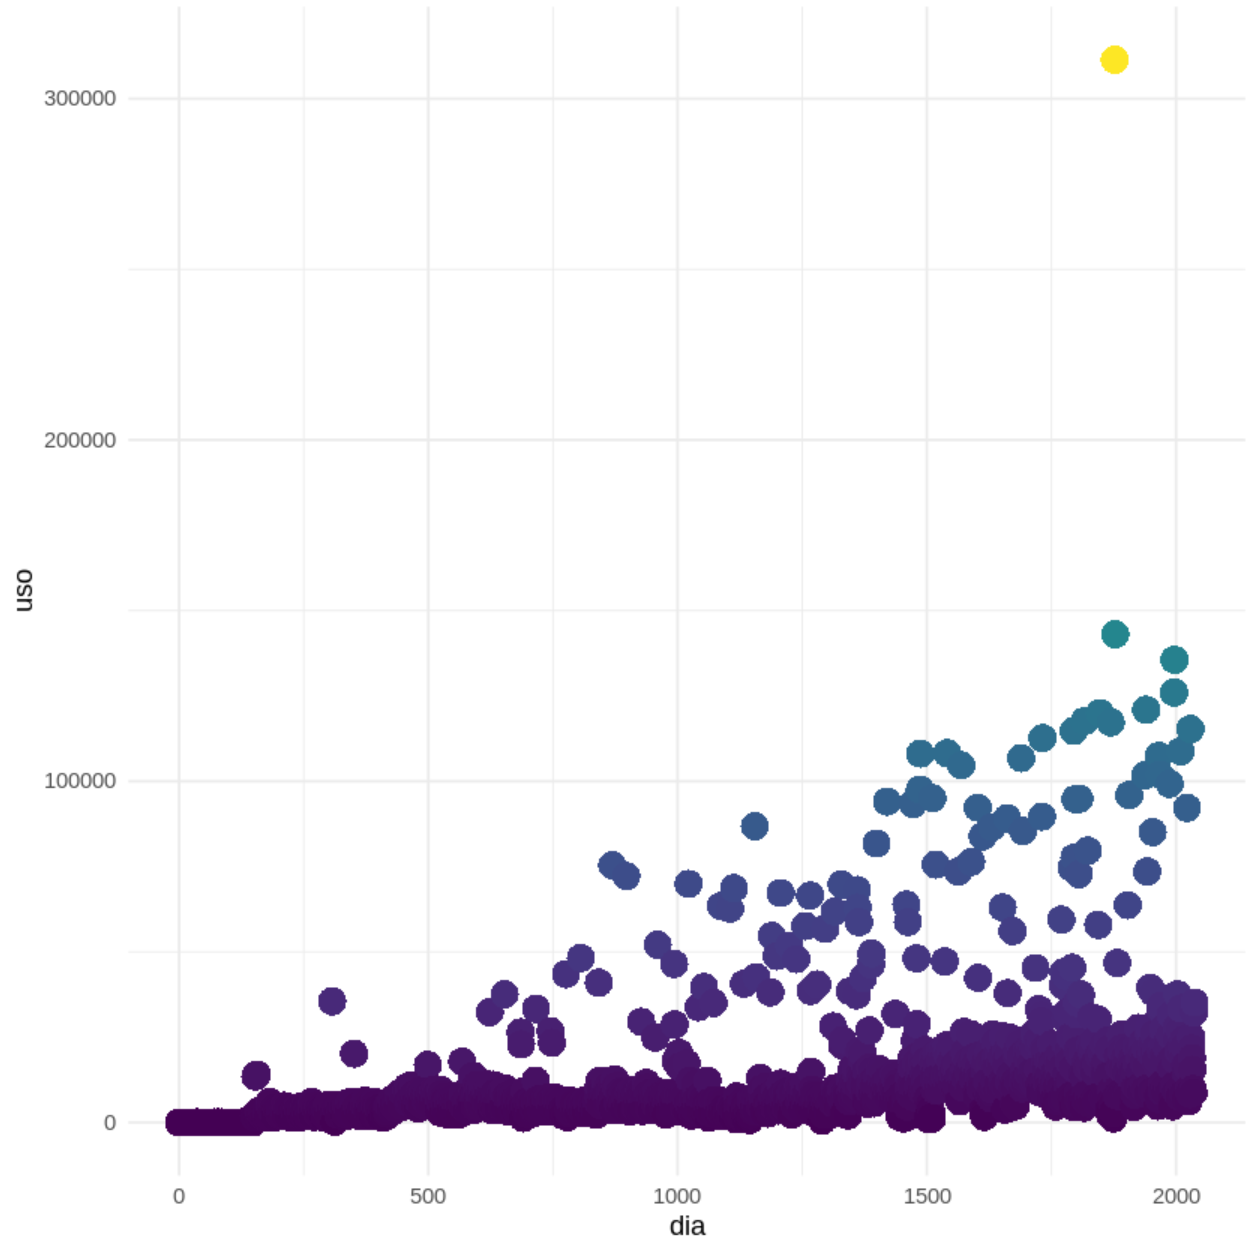
\includegraphics[scale=0.45]{RNL_00.png}
     \caption{Dados Plotados.}
     \label{figDados}
\end{figure}

\begin{figure}[h!tb]
     \centering
     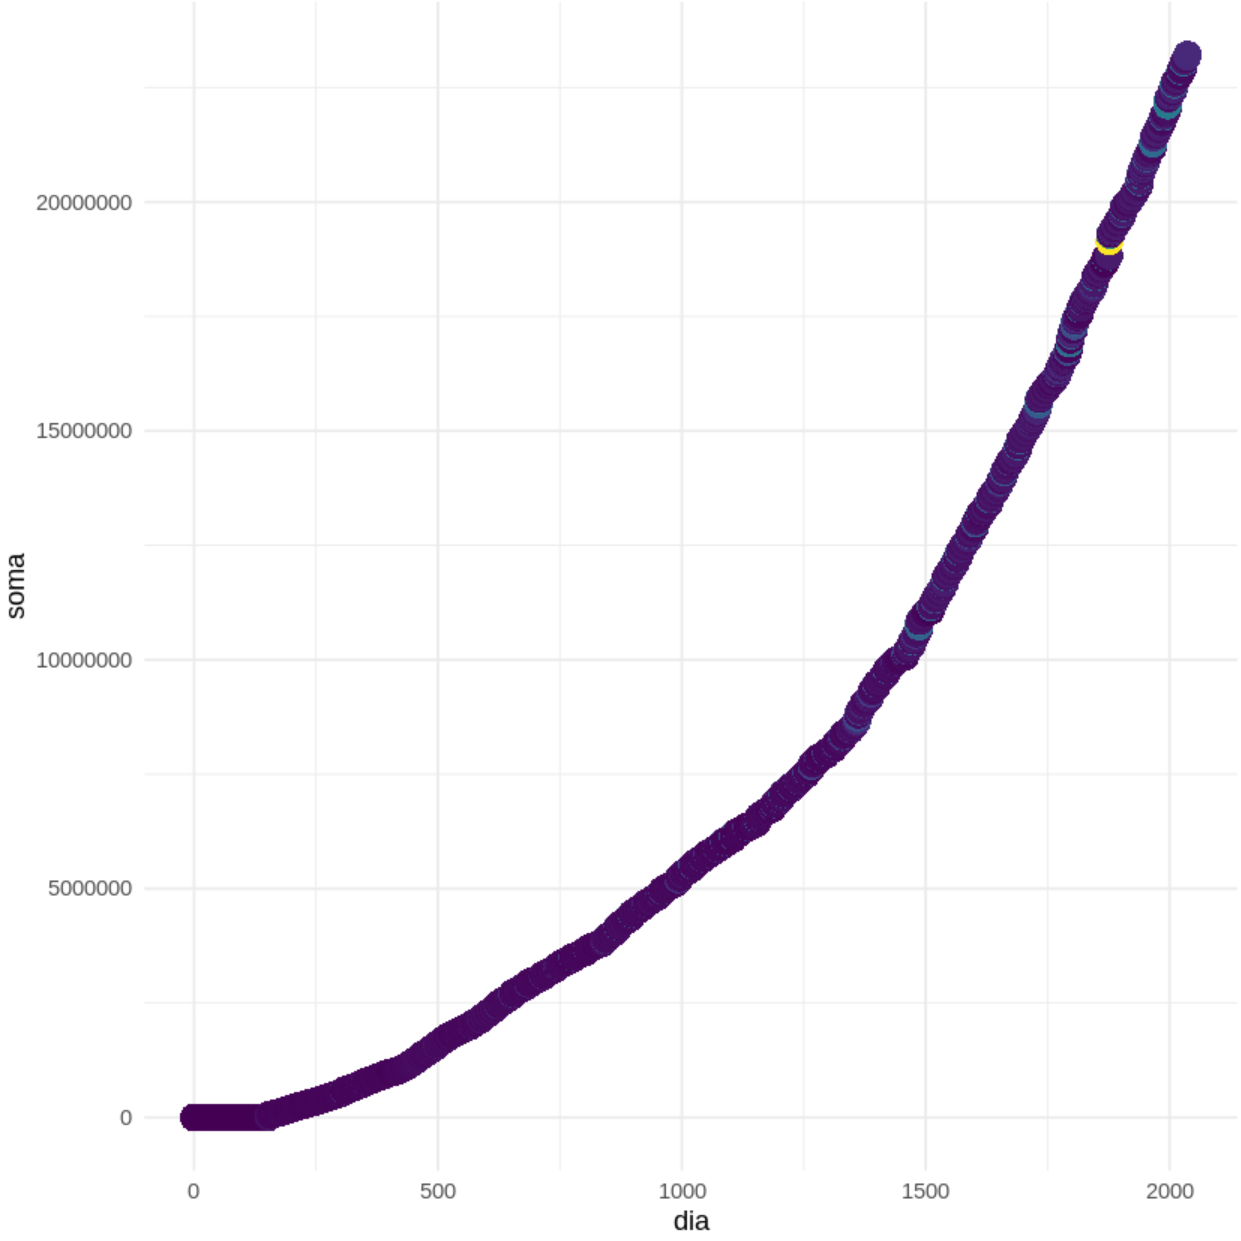
\includegraphics[scale=0.45]{RNL_01.png}
     \caption{Usos Acumulados.}
     \label{figAcum}
\end{figure}

\begin{figure}[h!tb]
     \centering
     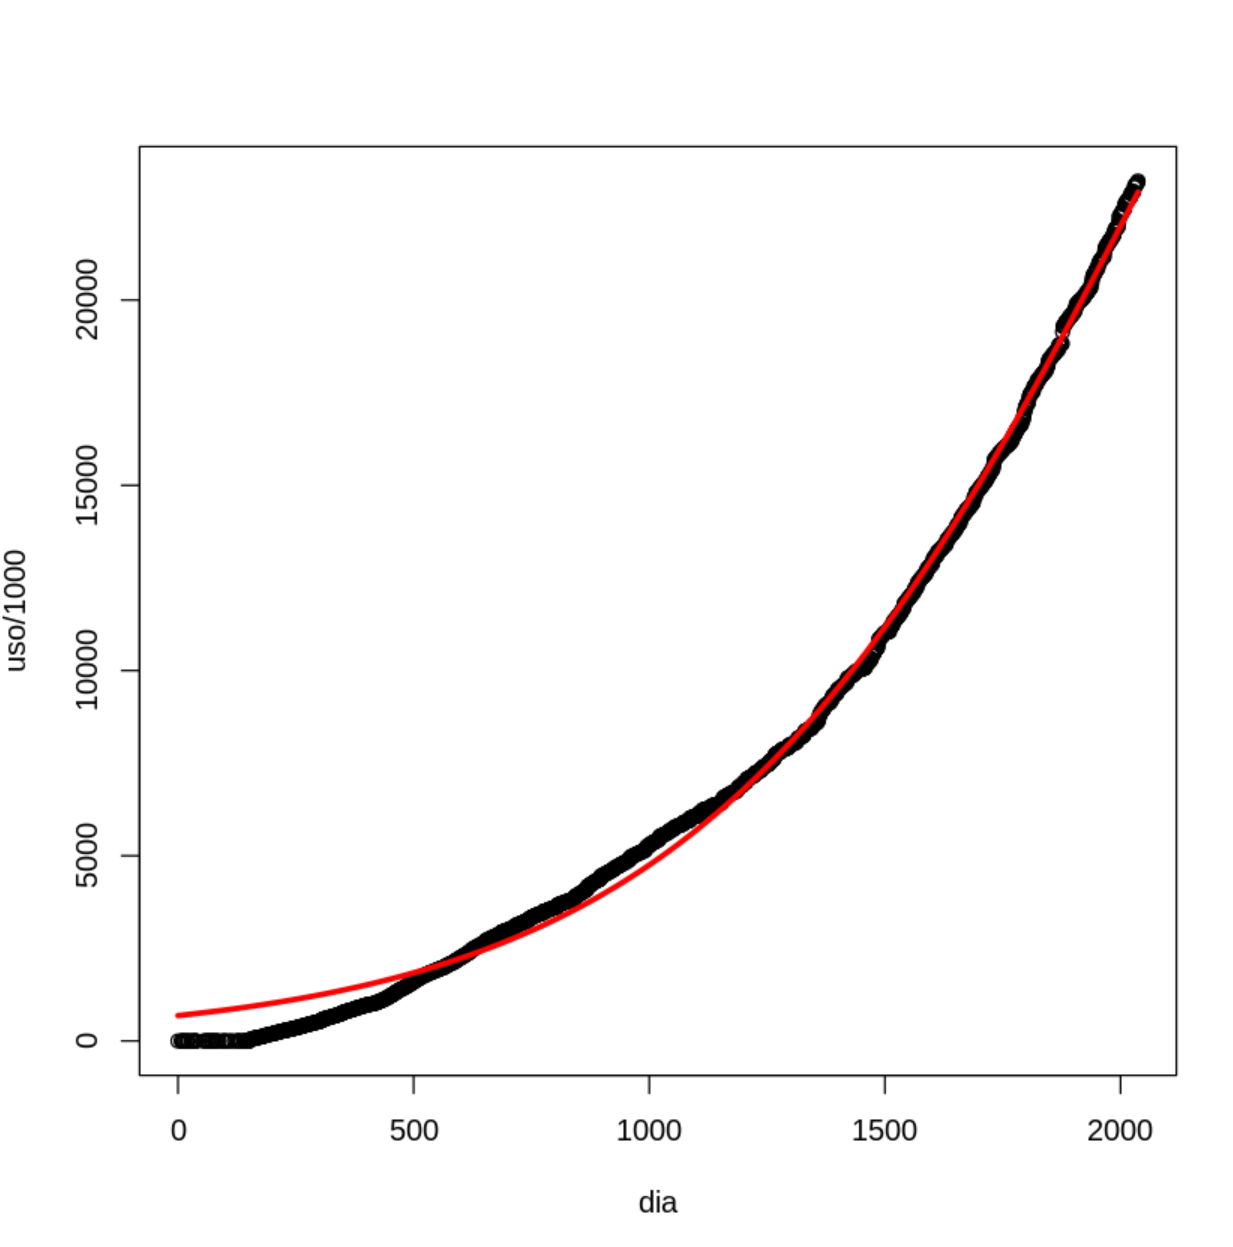
\includegraphics[scale=0.45]{RNL_02.png}
     \caption{Verificação do ajuste do Modelo.}
     \label{figAjs}
\end{figure}

\begin{figure}[h!tb]
     \centering
     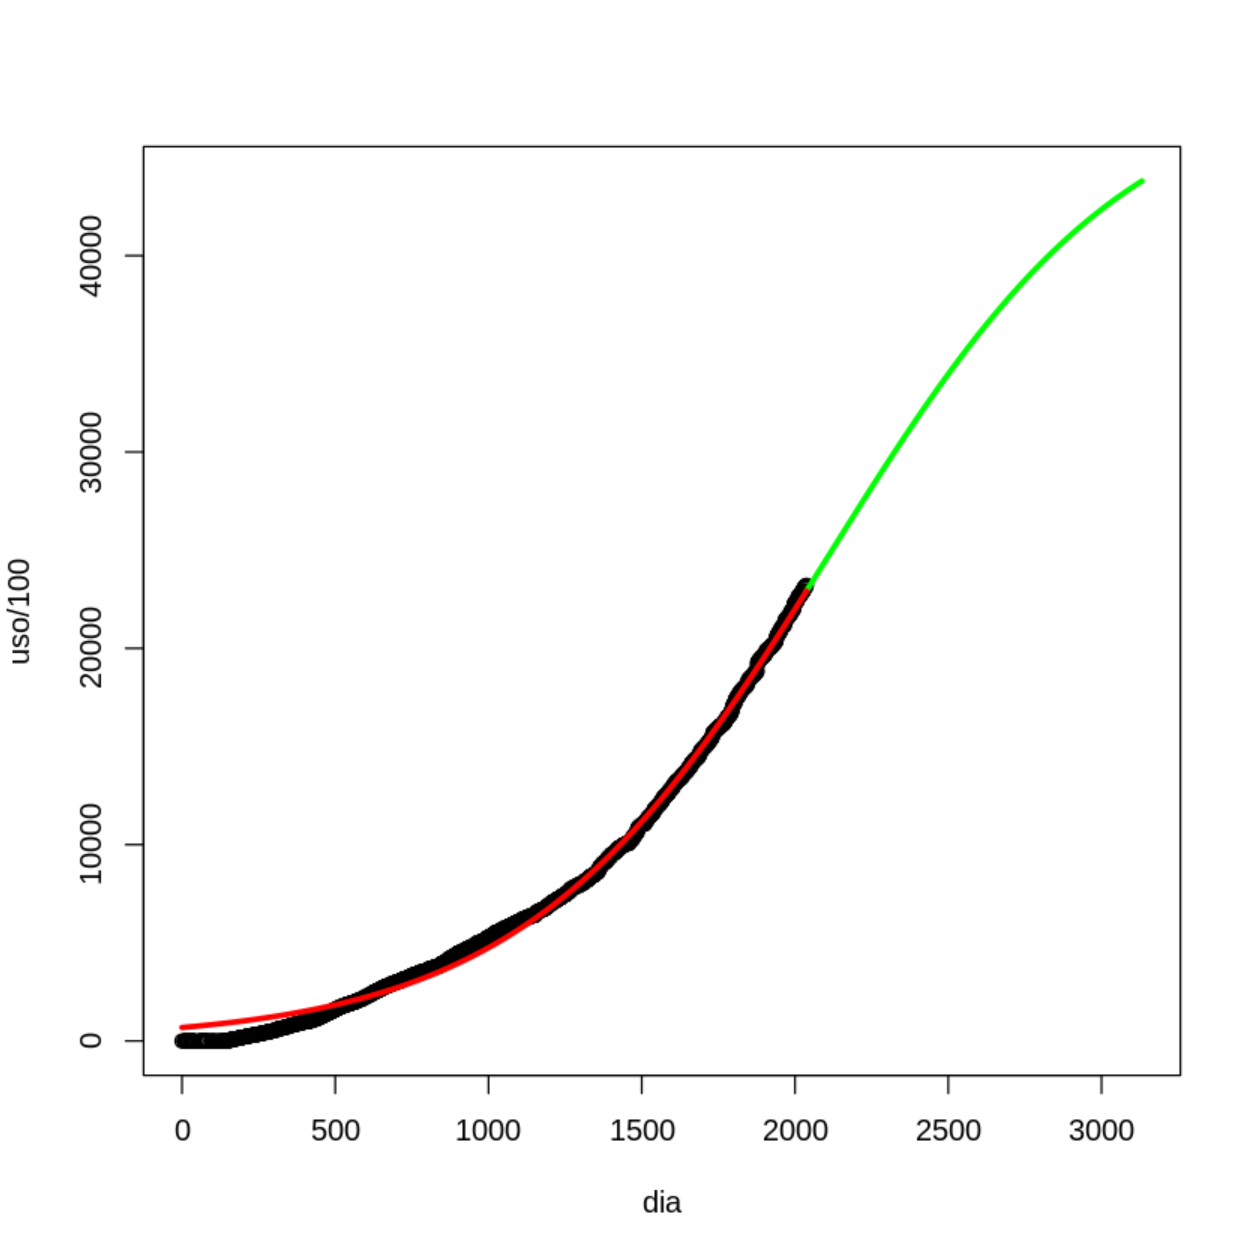
\includegraphics[scale=0.45]{RNL_03.png}
     \caption{Previsão do Modelo}
     \label{figModel}
\end{figure}

\end{document}


